\documentclass[tikz]{standalone}
\usepackage{calc}
\usepackage{braket}
% \usepackage{tikz}
\usetikzlibrary{arrows,backgrounds,positioning}
\usetikzlibrary{calc,math,fit,shapes,intersections}%<- added intersections
\usetikzlibrary{decorations.pathmorphing}
\pgfdeclarelayer{subbg}    % declare background layer
\pgfdeclarelayer{bg}    % declare background layer
\pgfdeclarelayer{bgmain}    % declare background layer
\pgfsetlayers{subbg,bg,bgmain,main}  % set the order of the layers (main is the standard layer)
% \usetikzlibrary{external}
% \tikzexternalize[prefix=external/]

\usepackage{xcolor}
\makeatletter % from https://tex.stackexchange.com/a/412901/121799
\newcommand{\Distance}[3]{% % from https://tex.stackexchange.com/q/56353/121799
\tikz@scan@one@point\pgfutil@firstofone($#1-#2$)\relax  
\pgfmathsetmacro{#3}{veclen(\the\pgf@x,\the\pgf@y)/28.45274}
}\makeatother 

% from https://tex.stackexchange.com/a/75084/121799
\newcommand\ellipsebyfoci[4]{% options, focus pt1, focus pt2, cste
  \path[#1] let \p1=(#2), \p2=(#3), \p3=($(\p1)!.5!(\p2)$)
  in \pgfextra{
    \pgfmathsetmacro{\angle}{atan2(\y2-\y1,\x2-\x1)}
    \pgfmathsetmacro{\focal}{veclen(\x2-\x1,\y2-\y1)/2/1cm}
    \pgfmathsetmacro{\lentotcm}{\focal*2*#4}
    \pgfmathsetmacro{\axeone}{(\lentotcm - 2 * \focal)/2+\focal}
    \pgfmathsetmacro{\axetwo}{sqrt((\lentotcm/2)*(\lentotcm/2)-\focal*\focal}
  }
  (\p3) ellipse[x radius=\axeone cm,y radius=\axetwo cm, rotate=\angle]{};
}

\newcommand\ellipticnode[6][]{% options, focus pt1, focus pt2, cste, name, value
 \pgfmathanglebetweenpoints{\pgfpointanchor{#2}{center}}
                            {\pgfpointanchor{#3}{center}}
 \edef\angle{\pgfmathresult} % save result in \angle 
 \Distance{(#2)}{(#3)}{\focal}
 \pgfmathsetmacro{\lentotcm}{\focal*#4}
 \pgfmathsetmacro{\axeone}{2*((\lentotcm - \focal)/2+\focal/2)}
 \pgfmathsetmacro{\axetwo}{2*(sqrt((\lentotcm/2)*(\lentotcm/2)-\focal*\focal/4)}
 \node at ($(#2)!.5!(#3)$) [shape=ellipse,minimum width=\axeone cm,minimum
 height=\axetwo cm, rotate=\angle,label=center:#6,#1] (#5)
  {};
}

\newcommand\ellipsenodebyfoci[6]{% options, focus pt1, focus pt2, cste, nodename, node content
  \path[#1] let \p1=(#2), \p2=(#3), \p3=($(\p1)!.5!(\p2)$)
  in \pgfextra{
    \pgfmathsetmacro{\angle}{atan2(\y2-\y1,\x2-\x1)}
    \pgfmathsetmacro{\focal}{veclen(\x2-\x1,\y2-\y1)/2/1cm}
    \pgfmathsetmacro{\lentotcm}{\focal*2*#4}
    \pgfmathsetmacro{\axeone}{(\lentotcm - 2 * \focal)/2+\focal}
    \pgfmathsetmacro{\axetwo}{sqrt((\lentotcm/2)*(\lentotcm/2)-\focal*\focal}
  }
  (\p3) node(#5) {#6} ellipse[x radius=\axeone cm,y radius=\axetwo cm, rotate=\angle];
}

\newcommand\fitEllipse[3]{% options, focus pt1, focus pt2
  \pgfmathanglebetweenpoints{\pgfpointanchor{#2}{center}}
  {\pgfpointanchor{#3}{center}}
 \edef\angle{\pgfmathresult} % save result in \angle 
  \node[rotate fit=\angle, fit=(#2)(#3),ellipse,#1]{};
}

\begin{document}

\tikzset{global scalea/.style={
    scale=#1,
    every node/.style={
      transform shape
      % scale=#1
    }
  }
}

% \tikzset{global scale/.style={
%     transform canvas={scale=#1}
% }

\tikzset{
  double arrow/.style args={#1 colored by #2 and #3}{
    -stealth,line width=#1,#2, % first arrow
    postaction={draw,-latex,#3,line width=(#1)/3,
                shorten <=(#1)/3,shorten >=2*(#1)/3}, % second arrow
  }
}


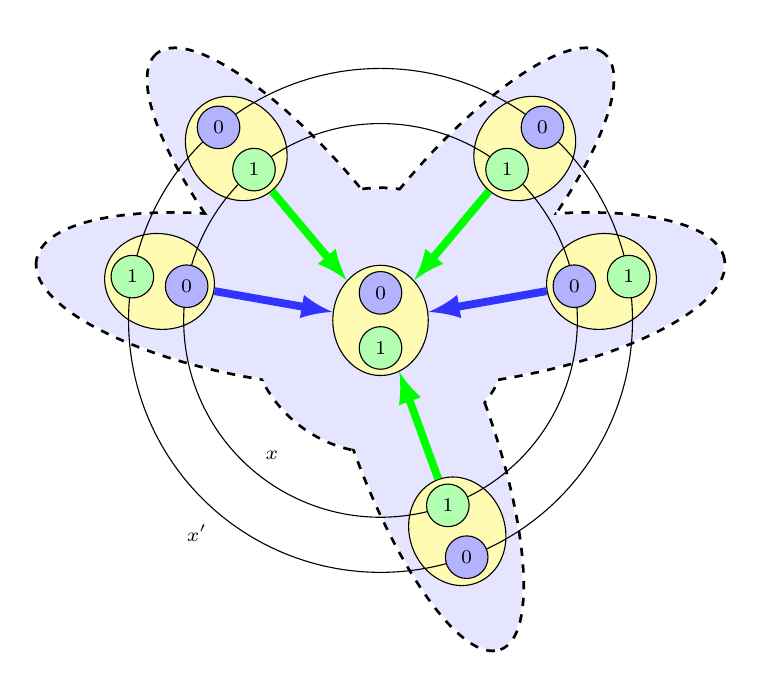
\begin{tikzpicture}
  \def\textSize{\scriptsize};
  \tikzmath{
    %%%%%%%%% Parameters
    int \n, \i, \s, \dispBigQubits, \dispCirc, \dispUseless;
    int \dispAlpha, \dispDashedGroup, \dispUselessArrows, \dispCentralTheta;
    int \dispBits, \dispCircleName;
    \n = 9;
    let \radiusFirst = 2.5cm;
    let \sizeEmptyQubit = .7cm;
    let \radiusSecond = \radiusFirst + \sizeEmptyQubit;
    let \marginFirst = 0;
    let \marginSecond = 0;
    \dispBigQubits = 1;
    % if dispBits = 2, then it's displays some eyes instead of the bits
    \dispBits = 1;
    \dispCirc = 1;
    \dispUseless = 0;
    \dispAlpha = 0;
    \dispDashedGroup = 1;
    \dispUselessArrows = 0;
    \dispCentralTheta = 0;
    \dispCircleName = 1;
    % Colors
    let \colorCentralQubit = orange!30;
    let \colorBitZero = blue!30;
    let \colorBitOne = green!30;
    let \colorSameBit = red!30;
    let \colorDiffBit = yellow!30;
    let \colorPlusArrow = green;
    let \colorMinusArrow = blue!80;
    let \colorDashedGroup = blue!10;
    % Values of qubits
    \i = 1;
    for \v in {0,1,0,1,0,1,1,0,1,0}{
      \valuesFirst{\i} = \v;
      \i = \i + 1;
    };
    \i = 1;
    for \v in {0,0,1,1,0,0,1,1,0,0}{
      \valuesSecond{\i} = \v;
      \i = \i + 1;
    };
    %%%%%%%%% Drawing
    % Center node      
    if \dispBigQubits == 1 then {
      if \dispCentralTheta then {
        { \node[circle](phantoma) at (0,\sizeEmptyQubit/2) {\phantom{0}};
          \node[circle](phantomb) at (0,-\sizeEmptyQubit/2) {\phantom{1}};
          \begin{pgfonlayer}{bg}
            \ellipticnode[draw,fill=\colorCentralQubit]{phantoma}{phantomb}{2.0}{centernode}{\textSize $\ket{+_\theta}$}
          \end{pgfonlayer}
        };
      } else {
        { \node[draw,circle,fill=\colorBitZero](phantoma) at (0,\sizeEmptyQubit/2) {\textSize $0$};
          \node[draw,circle,fill=\colorBitOne](phantomb) at (0,-\sizeEmptyQubit/2) {\textSize $1$};
          \begin{pgfonlayer}{bg}
            \ellipticnode[draw,fill=\colorDiffBit]{phantoma}{phantomb}{2.0}{centernode}{}
          \end{pgfonlayer}
        };
      };
    } else {
      { \node[circle, draw, fill=\colorCentralQubit,
        label=center:\textSize $\ket{+_\theta}$,
        minimum width=\sizeEmptyQubit,
        minimum height=\sizeEmptyQubit](centernode) at (0,0) {};};
    };
    if \dispBigQubits == 1 then {
      % Draw the first qubits
      for \s in {1,...,\n}{
        if \valuesFirst{\s} != \valuesSecond{\s} || \dispUseless == 1 then {
          if \valuesFirst{\s} == 1 then {let \ccolor = \colorBitOne;}
          else {let \ccolor = \colorBitZero;};
          if \dispBits == 1 then {
            { \node[draw, circle,fill=\ccolor]
              (first-\s) at ({90+360/\n * (\s - 1)}:\radiusFirst)
              {\textSize $\valuesFirst{\s}$};
            };
          } else {
            { \node[]
              (first-\s) at ({90+360/\n * (\s - 1)}:\radiusFirst)
              {\phantom{\textSize $\valuesFirst{\s}$}};
            };
          };
        };
        if \dispCirc then {
          { \begin{pgfonlayer}{bgmain}
              \draw[-] ({90+360/\n * (\s - 1)+\marginFirst}:\radiusFirst) 
              arc ({90+360/\n * (\s - 1)+\marginFirst}:{90+360/\n * (\s)-\marginFirst}:\radiusFirst);
            \end{pgfonlayer}};
        };
      };
      % Draw the second qubits
      for \s in {1,...,\n}{
        if \valuesFirst{\s} != \valuesSecond{\s} || \dispUseless == 1 then {
          if \valuesSecond{\s} == 1 then {let \ccolor = \colorBitOne;}
          else {let \ccolor = \colorBitZero;};
          if \dispBits == 1 then {
            { \node[draw, circle,fill=\ccolor]
              (second-\s) at ({90+360/\n * (\s - 1)}:\radiusSecond)
              {\textSize $\valuesSecond{\s}$};
            };
          } else {
            { \node[]
              (second-\s) at ({90+360/\n * (\s - 1)}:\radiusSecond)
              {\phantom{\textSize $\valuesSecond{\s}$}};
            };
          };
        };
        if \dispCirc then {
          { \begin{pgfonlayer}{bgmain}
              \draw[-] ({90+360/\n * (\s - 1)+\marginSecond}:\radiusSecond) 
              arc ({90+360/\n * (\s - 1)+\marginSecond}:{90+360/\n * (\s)-\marginSecond}:\radiusSecond);
            \end{pgfonlayer}};
        };
      };
      % Draw the eye
      for \s in {1,...,\n}{
        if \dispBits == 2 && \valuesFirst{\s} != \valuesSecond{\s} then {
          { \node[inner sep=0pt]
            (eye-\s) at ($(first-\s)!.5!(second-\s)$)
            {\includegraphics[width=\sizeEmptyQubit*\real{1}]{pictures/eye.pdf}};
          };
        };
      };
      % Draw the circle names
      if \dispCircleName && \dispCirc then {
        { \node[inner sep=0pt,label distance=.1mm, label=above right:\textSize $x$]
          (name-circle-1) at ({90+360/\n * 3.5}:\radiusFirst)
          {};
          \node[inner sep=0pt,label={[label distance=0mm]below left:\textSize $x'$}]
          (name-circle-2) at ({90+360/\n * 3.5}:\radiusSecond)
          {};
        };
      };
    };
    % Draw the ellipses
    for \s in {1,...,\n}{
      \vF = \valuesFirst{\s};
      \vS = \valuesSecond{\s};
      if \vF != \vS || \dispUseless == 1 then {
        if \vF == \vS then {let \ccolor = \colorSameBit; }
        else {let \ccolor = \colorDiffBit;};
        if \dispBigQubits == 1 then {
          { \begin{pgfonlayer}{bg}
              \ellipticnode[draw,fill=\ccolor]{first-\s}{second-\s}{2.0}{qubit-\s}{}
              % \node[fit=(first-\s)(second-\s), draw, circle, fill=\ccolor] {};
            \end{pgfonlayer}};
        } else {
          {
            \node[draw, circle,fill=\ccolor, minimum width=\sizeEmptyQubit, minimum height=\sizeEmptyQubit]
            (qubit-\s) at ({90+360/\n * (\s - 1)}:\radiusSecond)
            {};
          };
        };
      };
    };
    for \s in {1,...,\n}{
      % Draw the lines to the center
      \vF = \valuesFirst{\s};
      \vS = \valuesSecond{\s};
      if \vF != \vS then {
        if \vF == 1 then
        {
          let \sign = +;
          let \ccolor = \colorPlusArrow;
        }
        else
        {
          let \ccolor = \colorMinusArrow;
          let \sign = -;
        };
        if \dispAlpha == 1 then {
          { \draw[-latex,draw=\ccolor] (qubit-\s) -- (centernode)
            node[midway,fill=white,circle,draw=\ccolor]
            {\textSize $\textcolor{\ccolor}{\sign}\alpha_\s$};};
        } else {
          {
            \draw[-latex,draw=\ccolor,line width=1mm] (qubit-\s) -- (centernode);};
        };
      } else {
        if \dispUselessArrows && \dispUseless then {
          {\draw[-latex,dashed] (qubit-\s) -- (centernode);};
        };
      };
    };
    % Draw the dashed group
    if \dispDashedGroup then
    {
      { \begin{pgfonlayer}{subbg} };
        % First draw
        {\draw[dashed,line width=2pt] (0,0) circle (\radiusFirst*2/3);};
        for \s in {1,...,\n}{
          if \valuesFirst{\s} != \valuesSecond{\s} then {
            {
              \fitEllipse{inner sep=0pt,draw,dashed,line width=2pt}{centernode}{qubit-\s}
            };
          };
        };
        % Then fill
        {\path[fill=\colorDashedGroup] (0,0) circle (\radiusFirst*2/3);};
        for \s in {1,...,\n}{
          if \valuesFirst{\s} != \valuesSecond{\s} then {
            {
              \fitEllipse{inner sep=0pt,fill=\colorDashedGroup}{centernode}{qubit-\s}
            };
          };
        };
        {\end{pgfonlayer}};
    };
  }
\end{tikzpicture}

\end{document}

%%% Local Variables:
%%% mode: latex
%%% TeX-master: t
%%% End:
